\documentclass[xcolor=pdftex,x11names,table,hyperref]{beamer}

\usepackage{verbatim}
\usepackage{setspace}
\usepackage{url}
\usepackage{amstext}    % defines the \text command
\usepackage{array}		% for math mode tabulars
\usepackage{xcolor} % See documentation PDF at http://www.ctan.org/pkg/xcolor
\definecolor{darkgreen}{rgb}{0,0.3,0}
\definecolor{darkblue}{rgb}{.05,.05,.30}
\definecolor{lightgrey}{rgb}{0.65,0.65,0.65}
\usepackage{tikzsymbols}
\usepackage{tikz-qtree}


\setbeamertemplate{section in toc}[sections numbered]
\setbeamertemplate{subsection in toc}[subsections numbered]
\setbeamertemplate{subsubsection in toc}[subsubsections numbered]
\usetheme{Singapore}
\setbeamertemplate{navigation symbols}{}
\setbeamertemplate{footline}{%
\vspace{0.0em}%
\hspace{0.5em}%
{\color[rgb]{.1,.1,.1} \insertframenumber{}~/~\inserttotalframenumber}
}

\newcommand{\code}[1]{{\color{darkgreen}\texttt{#1}}}
\newcommand{\detail}[1]{{\color{lightgrey}\small{}#1}}
\newcommand{\teeny}[1]{\scalebox{0.09}{#1}}
\newcommand{\tablecolors}{\rowcolors{2}{blue!12}{white}} % Cool table colors


\begin{document}

\title{Probabilistic Context-free Grammars \\and Other Syntactic Language Models \\[1.5em]
 %\includegraphics[width=0.45\textwidth,angle=180]{images/15118-illustration-of-a-tree-silhouette-pv.png} \\[-1.0em]
 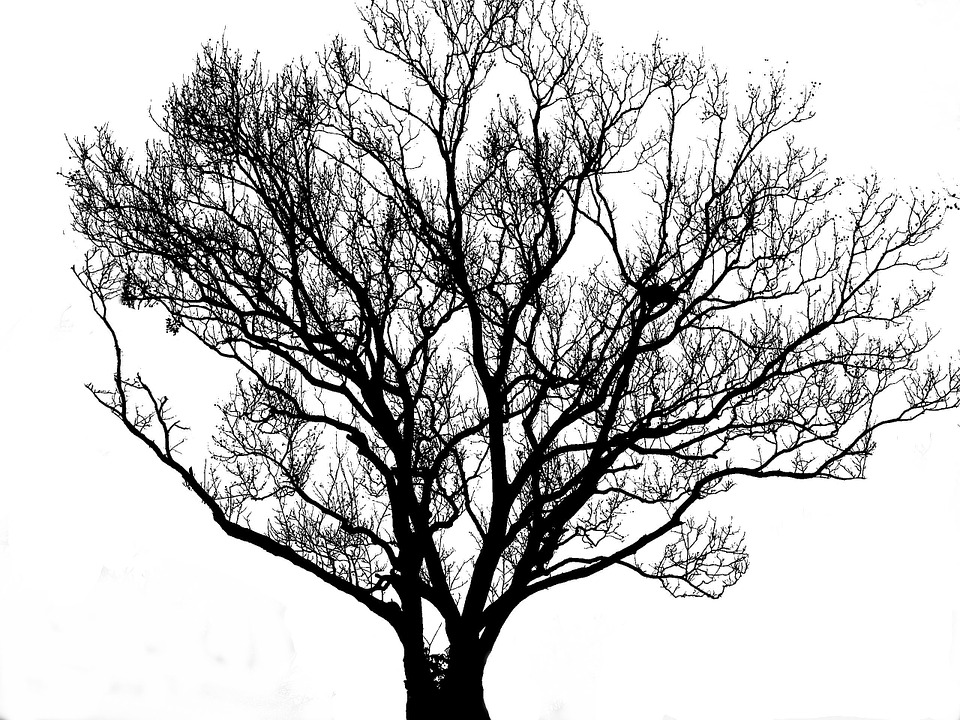
\includegraphics[height=0.35\textheight,angle=180]{images/tree-169250_960_720.jpg} \\[-1.0em]
 %\small{Possibilities} \\[1.0em]
 %LT1 \\[1.0em]
 }
\author{\href{http://jon.dehdari.org}{Jon Dehdari}}
\frame{\titlepage}

\begin{frame}{Kelsey and other Grammers}
\begin{itemize}
	\item A \textbf{grammar} here is another word for a language model
	\item They consist of four sets \detail{$G = \langle \Sigma, N, S, P \rangle$}
		\begin{description}
			\item[terminals] -- word types; lowest nodes in syntax trees \\ Examples: \textit{dog, the, eats}
			\item[non-terminals] -- phrasal types;  middle nodes in syntax trees \\ Examples: \textit{VP, DET, NP}
			\item[start symbol] -- ``S''; the top node in syntax trees
			\pause
		\item[production rules] -- recursive symbol substitutions \\ Examples:
		\end{description}
		\vspace{-1.0em}
		\begin{footnotesize}
		\begin{spacing}{0.6}
		\begin{align*}
			S & \rightarrow NP \ VP \\
			NP & \rightarrow DET \ N \\
			NP & \rightarrow ADJ \ N \\
			VP & \rightarrow V \ NP \\
			VP & \rightarrow V \\
			N & \rightarrow dog \\
			N & \rightarrow cat \\
			V & \rightarrow barks \\
			DET & \rightarrow the \\
		\end{align*}
		\end{spacing}
		\end{footnotesize}
\end{itemize}
\end{frame}

\begin{frame}{Visualization}
\begin{itemize}
	\item Sentences are often visualized using \textbf{derivation trees}, also known as \textbf{parse trees} or \textbf{syntax trees}
	\item Example: \\
		\begin{scriptsize}
		\tikzset{level distance=2.0em}
		\begin{tabular}{ll}
			\Tree [.S [.NP [.DET the ] [.N cat ] ][.VP [.V sat ][.PP [.P on ][.NP [.DET the ] [.N mat ] ] ] ] ] & %
		\pause
		\begin{minipage}{0.45\textwidth}
		\begin{spacing}{0.9}
		\begin{eqnarray*}
			S & \rightarrow & NP \ VP \\
			NP & \rightarrow & DET \ N \\
			DET & \rightarrow & the \\
			N & \rightarrow & cat \\
			VP & \rightarrow & V \ PP \\
			V & \rightarrow & sat \\
			PP & \rightarrow & P \ NP \\
			N & \rightarrow & mat
		\end{eqnarray*}
		\end{spacing}
		\vspace{-10.0em}
		\end{minipage}
		\end{tabular}
		\end{scriptsize}
	\pause
	\item Originally these trees were \textbf{mere visualizations} of how you could generate a grammatical sentence, given a grammar
	\pause
	\item Then people started to think of these trees as the actual \textbf{structure} of a sentence
	\pause
	\item Confusion ensued
\end{itemize}
\end{frame}

\begin{frame}{Context-free Grammars}
\begin{itemize}
	\item A \textbf{context-free grammar} (CFG) is a generative model that can generate context-free languages, which are somewhere in the middle of the formal language hierarchy
	\item Many, but not all, phenomena in natural languages can be generated by CFGs
	\pause
	\item Context-free production rules have the general form of a non-termal rewriting to a sequence (string) of terminals and/or non-terminals \detail{($A \rightarrow \alpha$)}
	\pause
	\item CFGs can generate and recognize \textbf{center embedding}, but not more complex word order phenomena, so effectively CFG parse trees have \textbf{no crossing lines}
	\pause
	\item Non-projective dependency grammars are more or less equivalent to CFGs \detail{(they have the same weak generative capacity)}
\end{itemize}
\end{frame}


\begin{frame}{Treebanks}
\begin{itemize}
	\item It's a lot of work to define a language model by hand (including context-free grammars), so another way is to annotate treebanks
	\item Example:
			(S (NP (DET the) (N cat))(VP (V sat)(PP (P on)(NP (DET the) (N mat)))))
	\pause
	\item There are treebanks for about 10--20 languages, the Penn Treebank being the most well-known for English
	\pause
	\item Treebanks can be annotated with various grammatical annotations, like \textbf{constituency / phrase-structure} (as above), \textbf{dependency grammar} (as we saw last class), categorial grammar, HPSG, etc.
	\item Most of these annotation styles can be approximately mapped to other styles
	\pause
	\item \href{https://en.wikipedia.org/wiki/Treebank\#Syntactic_treebanks}{Here is a link to a list of syntactic treebanks} 
\end{itemize}
\end{frame}


\begin{frame}{PCFGs}
\begin{itemize}
	\item We can induce a \textbf{probabilistic context-free grammar} (PCFG) from the treebank
	\item With multiple annotated sentences, we can get probabilities for production rules. Example: \\
		\begin{center}
		\begin{footnotesize}
		\begin{spacing}{0.9}
		\begin{tabular}{ >{$}l<{$}  >{$}l<{$}  >{$}l<{$} }
			1.0 & S & \rightarrow NP \ VP \\
			\hline
			0.6 & NP & \rightarrow DET \ N \\
			0.4 & NP & \rightarrow ADJ \ N \\
			\hline
			0.7 & VP & \rightarrow V \ NP \\
			0.3 & VP & \rightarrow V \\
			\hline
			0.8 & N & \rightarrow dog \\
			0.2 & N & \rightarrow cat \\
			\hline
			1.0 & V & \rightarrow barks \\
			\hline
			1.0 & DET & \rightarrow the \\
		\end{tabular}
		\end{spacing}
		\end{footnotesize}
		\end{center}
	\pause
	\item Notice that the probabilities for each left-hand side must sum to one \detail{(unity)}
\end{itemize}
\end{frame}


% parameter estimation using inside-outside algo (cite)
\begin{frame}{Parameter Estimation}
\begin{itemize}
	\item So how do we get these probabilities?
	\item If we have a treebank, we can start with just counting how often productions occur (maximum likelihood estimation)
	\item If we don't have a treebank, we can still use unannotated text, using the \textbf{inside-outside algorithm}
\end{itemize}
\end{frame}

\begin{frame}{Inside-Outside Algorithm}
\begin{itemize}
	\item The inside-outside algorithm is just the expectation-maximization algorithm applied to trees
	\item It uses inside- and outside-probabilities
	\item ...
\end{itemize}
\end{frame}


% advantages, dis- over regular language models: not incremental, can handle long-distance deps & agreement

% deniz' syn. lm

\begin{frame}{}
\begin{itemize}
	\item 
	\item 
	\item 
\end{itemize}
\end{frame}



\begin{frame}{}
\begin{itemize}
	\item 
	\item 
	\item 
\end{itemize}
\end{frame}




% \begin{frame}{}
% \begin{itemize}
% 	\item 
% 	\item 
% 	\item 
% \end{itemize}
% \end{frame}


\end{document}
